\documentclass[compress,9pt]{beamer}

%%%%%%% PACKAGES %%%%%%%%%
\usepackage[french]{babel}
\usepackage[backend=biber,style=authoryear,bibstyle=authoryear,natbib=true,
giveninits=true,uniquename=false,uniquelist=false,maxcitenames=2,date=year,
maxbibnames=99,url=false]{biblatex}
\addbibresource{Thèse.bib}
\usepackage{tikz}
\usepackage[T1]{fontenc}
\usepackage[utf8]{inputenc}
\usepackage{amsfonts}
\usepackage{amssymb}
\usepackage{lmodern}
\usepackage[absolute,overlay]{textpos}
\usepackage{contour}
\usepackage{ulem}
\usepackage{xcolor}
\usepackage{newunicodechar}
\usepackage{multirow}
\usepackage{setspace}
\usepackage{pifont}
\usepackage{appendixnumberbeamer}
%\usepackage{animate}

%%%%%%% PARAMETERS %%%%%%%%%
	%%%%%% CITE PARAMETERS %%%%%%%%%%%
		\AtEveryCitekey{\clearfield{title}\clearfield{note}\clearfield{pages}\clearlist{location}					\clearlist{publisher}\clearname{editor}}
		\renewcommand*{\multicitedelim}{\\}
		\renewcommand{\footfullcite}[1]{\footnote[frame]{\fullcite{#1}}}
		\def\bibfont{\tiny}			% Réduit la taille de la police dans les références biblio
	%%%%%% THEME %%%%%%%%
		\usetheme{Madrid}
		\useoutertheme[subsection=false]{miniframes}
		\usefonttheme{structurebold}
		\usepackage{etoolbox}
		\makeatletter
		\patchcmd{\slideentry}{\advance\beamer@xpos by1\relax}{}{}{}
		\def\beamer@subsectionentry#1#2#3#4#5{\advance\beamer@xpos by1\relax}%
		\makeatother
		\definecolor{myblue}{RGB}{120,150,200}
		\usecolortheme[named=myblue]{structure}
		\beamertemplatenavigationsymbolsempty 
		\setbeamerfont{page number in head/foot}{size=\tiny}
		\setbeamerfont{section in head/foot}{size=\scriptsize}
		\setbeamerfont{section in toc}{size=\footnotesize}
		\setbeamerfont{subsection in toc}{size=\tiny}
		\setbeamerfont{frametitle}{size=\large}
		\setbeamerfont{block title}{size=\normalsize}
		\setbeamerfont{block body}{size=\normalsize}
		\setbeamertemplate{footline}[frame number]
%		\setbeamertemplate{footnote}{size=\tiny}
		\setbeamertemplate{footcite}{site=\tiny}
		\setbeamercovered{transparent}
	%%%% ??
	\newcommand{\cmark}{\ding{51}}
	\newcommand{\xmark}{\ding{55}}
	\newcommand\Wider[2][3em]{%
	\makebox[\linewidth][c]{%
	  \begin{minipage}{\dimexpr\textwidth+#1\relax}
	  \raggedright#2
	  \end{minipage}%
	  }%
	}
	
%%%%%%%% TITLE %%%%%%%%%
\title{Comment valoriser les données anciennes pour l’analyse fréquentielle des crues : application au Rhône à Beaucaire de 1500 à 2020}
\author{Mathieu LUCAS}
\date{3 juillet 2023}

%%%%%%%%% MAIN PART %%%%%%%%%%
\begin{document}

%%%%%% PAGE DE TITRE %%%%%%%%
{
\usebackgroundtemplate{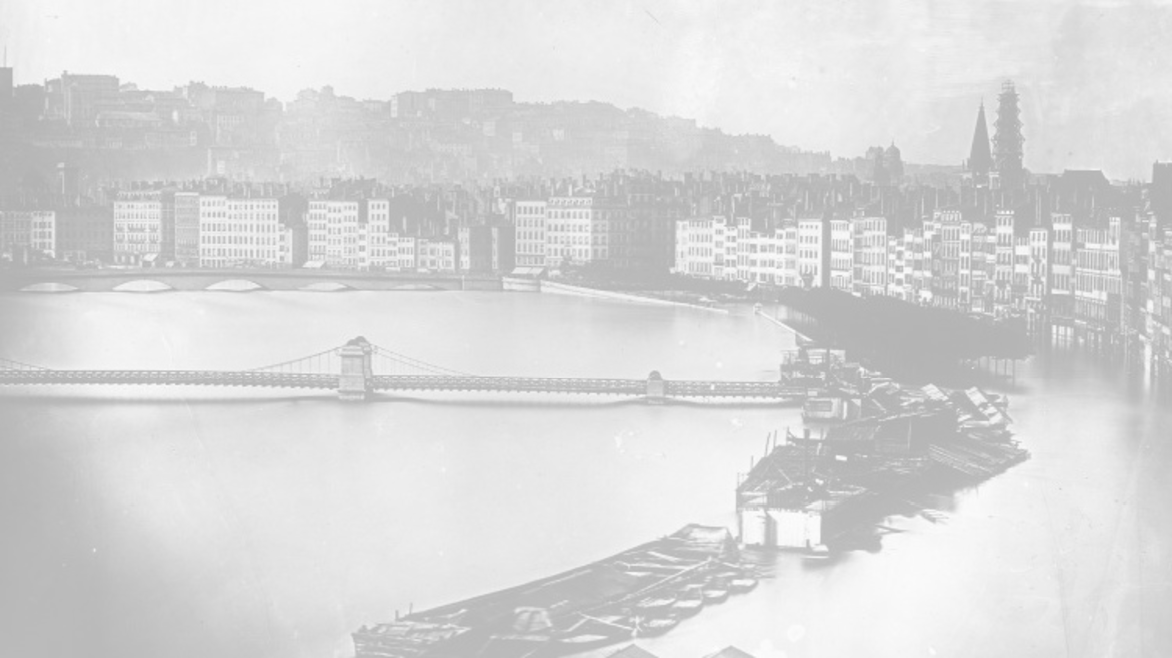
\includegraphics[height=\paperheight,width=\paperwidth]{./Figures/Back.pdf}}

\begin{frame}[plain]
     \vfill
     \centering

     \begin{beamercolorbox}[sep=8pt,center,colsep=-4bp,rounded=true,shadow=true]{institute}
     \end{beamercolorbox}
     {\usebeamercolor[fg]{titlegraphic}\inserttitlegraphic\par}
     \begin{beamercolorbox}[sep=12pt,center,colsep=-4bp,rounded=true,shadow=true]{title}
        \usebeamerfont{title}\inserttitle\par%
        \ifx\insertsubtitle\@empty%
        \else%
        \vskip0.25em%
        {\usebeamerfont{subtitle}\usebeamercolor[fg]{subtitle}\insertsubtitle\par}%
      \fi%     
     \end{beamercolorbox}%
     \vskip1em\par
     \begin{beamercolorbox}[sep=12pt,center,colsep=-4bp,rounded=true,shadow=true]{author}
%        \usebeamerfont{author}
        \Large{\insertauthor}
     \end{beamercolorbox}
    \begin{beamercolorbox}[sep=12pt,center,colsep=-4bp,rounded=true,shadow=true]{author}
   
%    \begin{center}
	    \begin{columns}[t]
	    	\begin{column}[t]{0.35\textwidth}
				\flushright{\small{Encadrement :}}
			\end{column}%
			\begin{column}{0.45\textwidth}
			\begin{flushleft}			
				\small{Michel LANG (INRAE RiverLy) \newline
				Jérôme LE COZ (INRAE RiverLy) \newline
				Benjamin RENARD (INRAE RECOVER)}
			\end{flushleft}
			\end{column}%
			\begin{column}{0.25\textwidth}
			\end{column}%
	    \end{columns}
%	\end{center}
	
%    \small{\underline{Encadrement} : Michel LANG (INRAE RiverLy) \newline
%    \textcolor{white}{Encadrement :} Jérôme LE COZ (INRAE RiverLy) \newline
%    \textcolor{white}{Encadrement :    } Benjamin RENARD  (INRAE RECOVER)}
    \end{beamercolorbox}
     \begin{beamercolorbox}[sep=8pt,center,colsep=-4bp,rounded=true,shadow=true]{date}
        \usebeamerfont{date}\insertdate
     \end{beamercolorbox}\vskip0.5em
% 	\vspace*{1cm}


%
%\begin{centering}
%\begin{columns}[b]
%\begin{column}{0.15\textwidth}
%\includegraphics[height=8mm]{./figures/intro/logoUGA.pdf} 
% \end{column}%
% \begin{column}{0.15\textwidth}
%  \textcolor{white}{bla}
% \end{column}
%\begin{column}{0.15\textwidth}
%\includegraphics[height=9mm]{./figures/intro/logoEDF.pdf} 
% \end{column}%
% \begin{column}{0.15\textwidth}
%  \textcolor{white}{bla}
% \end{column}
% \begin{column}{0.15\textwidth}
%\includegraphics[height=4mm]{./figures/intro/logoINRAE.pdf}
% \end{column}
%\end{columns}
%
%\end{centering}

\end{frame} 
}

\section{Introduction}
	\subsection{Le risque de crue}
	
	%%%%%%%%% 2 %%%%%%%%%
	\begin{frame}[c]
		\frametitle{Le risque de crue}
      	\begin{minipage}{0.49\textwidth}
      		Premier type de catastrophe naturelle dans le monde au XXI\textsuperscript{ème} siècle\footfullcite{undrr_human_2020} en terme de :
      		\vspace{10pt}
      		\begin{itemize}
      			\item<1->[$\vartriangleright$] Nombre d'occurrences
      			\vspace{10pt}
      			\item<2>[$\vartriangleright$] Nombre de personnes affectées
      		\end{itemize}
      	\end{minipage}
      	\hfill
      	\begin{minipage}{0.49\textwidth}
      		\begin{center}
				\item \includegraphics<1>[width= .9\textwidth]{./Figures/UNDRR.jpg}  
				\vspace{3pt}    	
				\item \includegraphics<2>[width = .9\textwidth]{./Figures/UNDRR-2.jpg} 
      		\end{center}
      	\end{minipage}
	\end{frame}
		
	\subsection{L'estimation du risque}
	%%%%%%%%% 3 %%%%%%%%%
	\begin{frame}%[c]
		\frametitle{L'estimation du risque}
      	\begin{minipage}{0.5\textwidth}
      		Nécessité de caractériser statistiquement l'aléa de crue :
      		\vspace{10pt}
      		\begin{itemize}
      			\item<2->[$\vartriangleright$] Plan de Prévention du Risque Inondation : \og\textit{déterminé à partir de l'événement le plus important connu ou d'un évènement théorique de \textbf{fréquence centennale}}[...]\fg{} \footfullcite{Code de l'environnement; article R562-11-3}
      			\vspace{10pt}
      			\item<3>[$\vartriangleright$] Dimensionnement d'infrastructures à risque (évacuateurs de crue, digues de protection...) : \textbf{périodes de retour jusqu'à 10 000 ans}
      		\end{itemize}
      	\end{minipage}
      	\begin{minipage}{0.45\textwidth}
      		\begin{center}
				\item \includegraphics<2>[width = .9\textwidth]{./Figures/PPRI_lyon.pdf}  
				\item \includegraphics<3>[width = .9\textwidth]{./Figures/Grangent.jpg} 
      		\end{center}
      	\end{minipage}
	\end{frame}
	
	
	%%%%%%%%% 4 %%%%%%%%%
	\begin{frame}%[c]
		\frametitle{L'estimation du risque}
      	\begin{minipage}{0.5\textwidth}
      		Nécessité de caractériser statistiquement l'aléa de crue :
      		\vspace{10pt}
      		\begin{itemize}
      			\item<2->[$\vartriangleright$] Plan de Prévention du Risque Inondation : \og\textit{déterminé à partir de l'événement le plus important connu ou d'un évènement théorique de \textbf{fréquence centennale}}[...]\fg{} \footfullcite{Code de l'environnement; article R562-11-3}
      			\vspace{10pt}
      			\item<3>[$\vartriangleright$] Dimensionnement d'infrastructures à risque (évacuateurs de crue, digues de protection...) : \textbf{débits de période de retour jusqu'à 10 000 ans}
      		\end{itemize}
      	\end{minipage}
      	\begin{minipage}{0.45\textwidth}
      		\begin{center}
				\item \includegraphics<2->[width = .9\textwidth]{./Figures/PPRI_lyon.pdf}  
				\item \includegraphics<3>[width = .9\textwidth]{./Figures/Grangent.jpg} 
      		\end{center}
      	\end{minipage}
	\end{frame}
	  
	\subsection{Crues et statistiques}
	%%%%%%%%% 5 %%%%%%%%%
	\begin{frame}%[c]
		\frametitle{Crues et probabilités}
      	crues = réalisations + concept de période de retour
	\end{frame}

	%%%%%%%%% 6 %%%%%%%%%
	\begin{frame}%[c]
		\frametitle{Crues et probabilités}
      	Estimation d'une distribution
	\end{frame}
	


\section{Le Rhône à Beaucaire}


\section{1816-2020}


\section{1500-2020}



\section{Conclusion}

	\subsection{Conclusion}
	\subsection{Perspectives}
	\subsection{Remerciements}
	
%\printbibliography
	
\section{Annexes}
	



%\begin{frame}{blabla}
%	\begin{itemize}
%			\item \footfullcite{steinbakk_propagation_2016}
%		
%	\end{itemize}
%	
%\end{frame}
%
%\begin{frame}
%		\printbibliography
%\end{frame}
%




\end{document}
